\documentclass[11pt,a4paper]{article}
\usepackage[T1]{fontenc}
\usepackage[utf8]{inputenc}
\usepackage[magyar]{babel}
\usepackage{lmodern}
\usepackage{amsmath}
\usepackage{enumitem}
\usepackage{tikz}
\usepackage[a4paper,margin=2cm]{geometry}

\pagestyle{empty}
\setlength{\parindent}{0pt}

\begin{document}

\begin{center}
{\large\bfseries Termodinamika -- állapotjelzők és folyamatjellemzők}

\vspace{6pt}
\fbox{\parbox{0.92\linewidth}{\centering
A feladatsorban a $\Delta E = Q + W$ alakot használjuk, ahol $W$ a \emph{gázon végzett} munka.}}
\end{center}

\vspace{2pt}

\begin{enumerate}[leftmargin=*,label=\textbf{\arabic*.},itemsep=8pt,topsep=0pt,parsep=0pt]

\item 
\textbf{a)} Lehet-e egy gáz hőmérsékletét növelni hőközlés nélkül? Ha igen, hogyan?
\textbf{b)} Lehet-e hőt közölni egy rendszerrel úgy, hogy a hőmérséklete ne
változzon? Adj két különböző példát!

\item
\begin{minipage}[t]{0.56\linewidth}
Egy ideális gáz az $A$ állapotból ($p_0$, $V_0$) a $B$ állapotba
($p_0/2$, $2V_0$) jut el kétféle úton:\\[2pt]
\textbf{I.~út:} előbb izobár tágulás $2V_0$-ig, majd izochor hűtés $p_0/2$-ig;\\
\textbf{II.~út:} előbb izochor hűtés $p_0/2$-ig, majd izobár tágulás $2V_0$-ig.\\[2pt]
\textbf{a)} Számold ki mindkét úton külön-külön a gázon végzett munkát és a gázzal
közölt hőt!
\textbf{b)} Számold ki mindkét úton a belső energia megváltozását!
\textbf{c)} Mit veszel észre? Melyik mennyiség függ az úttól, és melyik nem? Miért?
\end{minipage}\hfill
\begin{minipage}[t]{0.40\linewidth}
\vspace{0pt}
\centering
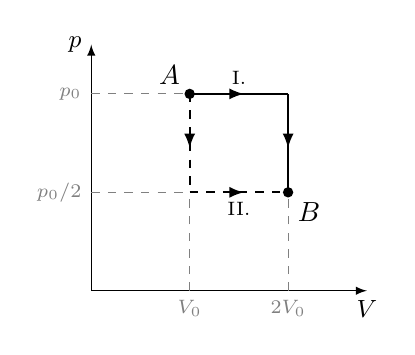
\begin{tikzpicture}[scale=1.25,>=latex]
  \draw[->] (0,0) -- (2.8,0) node[below] {\small $V$};
  \draw[->] (0,0) -- (0,2.5) node[left] {\small $p$};
  \draw[gray,dashed] (1,0) node[below] {\scriptsize $V_0$} -- (1,1);
  \draw[gray,dashed] (2,0) node[below] {\scriptsize $2V_0$} -- (2,1);
  \draw[gray,dashed] (0,2) node[left] {\scriptsize $p_0$} -- (1,2);
  \draw[gray,dashed] (0,1) node[left] {\scriptsize $p_0/2$} -- (1,1);
  % I. út
  \draw[thick,->] (1,2) -- (1.55,2);
  \draw[thick] (1.5,2) -- (2,2);
  \draw[thick,->] (2,2) -- (2,1.45);
  \draw[thick] (2,1.5) -- (2,1);
  \node[above] at (1.5,2) {\scriptsize I.};
  % II. út
  \draw[thick,dashed,->] (1,2) -- (1,1.45);
  \draw[thick,dashed] (1,1.5) -- (1,1);
  \draw[thick,dashed,->] (1,1) -- (1.55,1);
  \draw[thick,dashed] (1.5,1) -- (2,1);
  \node[below] at (1.5,1) {\scriptsize II.};
  \fill (1,2) circle (1.5pt) node[above left] {$A$};
  \fill (2,1) circle (1.5pt) node[below right] {$B$};
\end{tikzpicture}
\end{minipage}

\item Egy gázzal egymás után a következőket tesszük: izoterm tágulás, izochor
melegítés, adiabatikus összenyomás. Töltsd ki a táblázatot a $+$, $-$ vagy $0$
jelekkel! Minden cellához írj egymondatos indoklást, külön sorba a táblázat alá!

\vspace{6pt}
\begin{center}
\renewcommand{\arraystretch}{1.8}
\begin{tabular}{|l|c|c|c|c|}
\hline
\textbf{Folyamat} & \hspace{0.6cm}$\Delta T$\hspace{0.6cm} & \hspace{0.6cm}$\Delta E$\hspace{0.6cm}
  & \hspace{0.6cm}$W$\hspace{0.6cm} & \hspace{0.6cm}$Q$\hspace{0.6cm} \\ \hline
izoterm tágulás         & & & & \\ \hline
izochor melegítés       & & & & \\ \hline
adiabatikus összenyomás & & & & \\ \hline
\end{tabular}
\end{center}
\vspace{1.6cm}

\item Egy ideális gáz izobár folyamatát ábrázoltuk $p$--$V$ diagramon. Rajzold fel
ugyanezt a folyamatot $V$--$T$ és $p$--$T$ diagramon is! Jelöld a folyamat irányát
nyíllal!

\vspace{4pt}
\begin{center}
\begin{tikzpicture}[scale=0.8,>=latex]
  \draw[->] (0,0) -- (3.2,0) node[below] {\small $V$};
  \draw[->] (0,0) -- (0,2.4) node[left] {\small $p$};
  \draw[gray,dashed] (0,1.5) node[left] {\scriptsize $p_0$} -- (0.8,1.5);
  \draw[gray,dashed] (0.8,0) node[below] {\scriptsize $V_1$} -- (0.8,1.5);
  \draw[gray,dashed] (2.6,0) node[below] {\scriptsize $V_2$} -- (2.6,1.5);
  \draw[thick,->] (0.8,1.5) -- (1.75,1.5);
  \draw[thick] (1.7,1.5) -- (2.6,1.5);
  \fill (0.8,1.5) circle (1.5pt) node[above] {\scriptsize 1};
  \fill (2.6,1.5) circle (1.5pt) node[above] {\scriptsize 2};
\end{tikzpicture}
\hspace{1.2cm}
\begin{tikzpicture}[scale=0.8,>=latex]
  \draw[->] (0,0) -- (3.2,0) node[below] {\small $T$};
  \draw[->] (0,0) -- (0,2.4) node[left] {\small $V$};
\end{tikzpicture}
\hspace{1.2cm}
\begin{tikzpicture}[scale=0.8,>=latex]
  \draw[->] (0,0) -- (3.2,0) node[below] {\small $T$};
  \draw[->] (0,0) -- (0,2.4) node[left] {\small $p$};
\end{tikzpicture}
\end{center}

\item
\begin{minipage}[t]{0.55\linewidth}
$0\,^\circ$C-os jeget melegítünk, amíg $20\,^\circ$C-os víz nem lesz belőle.
Vázold fel a hőmérséklet--idő grafikont állandó teljesítményű fűtés mellett, és
magyarázd meg, mi történik a közölt hővel a vízszintes szakaszon!
\end{minipage}\hfill
\begin{minipage}[t]{0.40\linewidth}
\vspace{0pt}
\centering
\begin{tikzpicture}[scale=0.8,>=latex]
  \draw[->] (0,0) -- (4.2,0) node[below] {\small $t$};
  \draw[->] (0,-0.3) -- (0,2.4) node[left] {\small $T$\,($^\circ$C)};
  \draw (0.1,0) -- (-0.1,0) node[left] {\scriptsize 0};
  \draw (0.1,1.8) -- (-0.1,1.8) node[left] {\scriptsize 20};
\end{tikzpicture}
\end{minipage}

\end{enumerate}

\end{document}
